

\chapter{\selfour Basics}
\label{chap:sel4}

So far we have provided a general background on real-time scheduling and resource sharing.
Finally we will present an overview of the concepts relevant to the temporal behaviour of our implementation platform, \selfour.

\selfour is a microkernel that is particularly suited to safety-critical, real-time systems with one major caveat: the lack of real-time scheduling support. 
Three main features of \selfour support this claim: it has been formally verified for correctness~\citep{Klein_EHACDEEKNSTW_09} and other properties~\citep{Sewell_WGMAK_11}; All memory management, including kernel memory, is all at user-level~\citep{Elkaduwe_Derrin_06}; Finally it is the only \gls{OS} to date with full \gls{WCET} analysis~\citep{Blackham_SCRH_11}.
The scheduler in \selfour has been left intentionally underspecified~\citep{Petters_EH_12} for later work and as a result has a very informal notion of time.
The current implementation is a placeholder, and follows the traditional L4 scheduling model~\citep{Ruocco_06} --- a fixed-priority, round-robin scheduler with 256 priorities.

Systems can currently choose between a restrictive implementation of temporal isolation or a system that presents timing behaviour that is impossible to analyse beyond trivial examples\footnote{Whether analysis is possible in a trivial example beyond one thread is questionable.}.
In this section we will present the current state of relevant \selfour features in order to highlight deficiencies and motivate our changes.
We will outline the existing scheduler, the API curiosity that is \yield, and how \gls{IPC} interacts with scheduling, followed by an analysis of how the current mechanisms can be used in real-time systems.


\section{\selfour concepts}

First we introduce the basics of \selfour: kernel memory management, capabilities, \gls{IPC} and
signalling. \Cref{f:legend-1} shows the legend for diagrams in this section. 

\begin{figure}
    \centering
    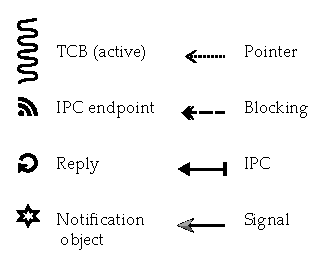
\includegraphics[width=0.5\textwidth]{legend-1}
    \caption{Legend for diagrams in this section}
    \label{f:legend-1}
\end{figure}

\subsection{Capabilities}
\label{s:capabilities}

As a capability-based \gls{OS}, access to any functionality in \selfour is via capabilities (recall
\Cref{s:capabilities}. Capabilities to all system resources are passed to the initial task --- the first
user level thread started in the system --- which can then allocate resources as appropriate.
Capabilities exist in a \emph{capability space} that can be configured per thread or shared between
threads. Capabilities spaces are analogous to address spaces for virtual memory, although
capabilities can be moved and copied between different spaces. 

All capabilities can be copied, potentially changing their access rights, except \emph{control}
capabilities, which can only be moved and not copied. Control capabilities provide the rights to do
specific operations, \eg the \emph{interrupt control} capability is used to obtain a capability
to a specific interrupt number.

Any individual capability can be deleted, or revoked. The former simply removes a specific
capability from a capability space, the latter removes all child capabilities.

% control caps, normal caps
% operations

\subsection{Kernel memory management}

All kernel memory in \selfour is managed at user-level and accessed via capabilities (recall
\Cref{s:capabilities}, which is key to \selfour's isolation and security, but also essential for
understanding the complexity of kernel design.

Capabilities to objects can be copied, which creates another capability to the same object,
potentially with different access rights, but not
a copy of the object itself. 
Similarly capabilities to objects can also be deleted, but only when the last capability to an
object is deleted will the object itself be deleted. Object capabilities contain a pointer to the
actual kernel object. 

All memory in \selfour starts as \emph{untyped} memory, capabilities to which is granted to the
initial task in the system as part of the boot process. The initial task can then create all
types of memory, including further untyped, with an operation known as \emph{retyping}. As a result,
any object with a pointer to another object must have a back pointer to update should that object be
deleted, in order to avoid stray pointers in the kernel. 

% table of object types 
\begin{table}
    \centering
    \rowcolors{2}{gray!25}{}
    \begin{tabular}{l p{0.6\textwidth}}\toprule
    \emph{Object}    & \emph{Description}\\\midrule
    CNode            & A fixed size table of capabilities, analogous to a page table in a virtual
                      memory system. \\
    \Gls{TCB}        & A thread of execution in \selfour.\\
    Endpoint  & Objects which facilitate \gls{IPC} between threads. \\
    Notification object & Objects which provide a signalling mechanism.\\
    VSpace     & A top level page table structure \\
    Interrupt & Allow access to specific hardware interrupts.\\
    Untyped    & Memory that can be retyped into other types of memory, including untyped.\\
    \bottomrule
    \end{tabular}
    \caption{Major object types in \selfour, excluding platform specific objects. For further detail
    consult the \selfour manual~\citep{seL417}}.
     \label{t:kernel_objects}
\end{table}

\Cref{t:kernel_objects} gives an overview of basic object types in \selfour. 
While the majority of objects in \selfour have a platform-dependant size fixed at compile time, some
are variably sized, \eg untyped and CNodes, which can be any power of two size, as custom

\subsection{Thread control blocks}

\Glspl{TCB} represent a unit of execution in \selfour and deviate from other object in that they
consist of the core \gls{TCB}, and a CNode which contains a capability to that threads CNode, vspace
and \gls{IPC} buffer.

\subsection{IPC}
\label{s:ipc}

\gls{IPC} is the microkernel mechanism for synchronous transmission of data and capabilities. In the \selfour model,
\gls{IPC} takes place via endpoints, which represent a general communication port. Any thread with a
capability to an endpoint can send and receive messages on that endpoint, subject to the access
rights. Most messages sent fit into registers, however messages exceeding this platform dependent
size are placed in the Messages sent via \gls{IPC} are stored in the \gls{IPC} buffer, a kernel-writeable frame per
thread. 

IPC can be one-way, where the sender blocks until the message is sent then may continue
(\texttt{send()} , or two-way,
where the sender blocks until a reply message is sent (\texttt{call()}. One-way IPC may also be
non-blocking, where the message is only sent of a receiver is already present.
Multiple senders and receivers can use the same endpoint, and which act as \gls{FIFO}
queues. 

\begin{figure}
    \centering
    \begin{subfigure}[h]{0.48\textwidth}
        \centering
        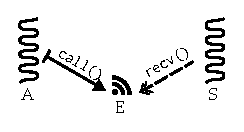
\includegraphics[width=\textwidth]{ipc1}
        \caption{Phase 1}
        \label{f:ipc1}
    \end{subfigure}%
    \begin{subfigure}[h]{0.48\textwidth}
        \centering
        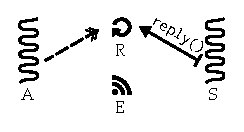
\includegraphics[width=\textwidth]{ipc2}
        \caption{Phase 2}
        \label{f:ipc2}
    \end{subfigure}
    \label{f:ipc}
    \caption{IPC phases: (a) shows the initial IPC rendezvous, (b) shows the
    reply phase. See \Cref{f:legend-1} for the legend.}
\end{figure}

Two-way IPC has two phases, as \cref{f:ipc} illustrates: rendezvous and reply.

\Cref{f:ipc1} demonstrates the rendezvous phase, where regardless of the order of operations, 
when one thread blocks (\cref{recv}) on the endpoint and another thread sends on that endpoint
then message is sent. This occurs for both one-way and two-way \gls{IPC}.

The reply phase, illustrated in \Cref{f:ipc2}, only occurs if the sender used \texttt{call} to send
the \gls{IPC}. In this case, a one-off \emph{resume} capability is generated, which the caller ($A$)
blocks on, and the receiver ($S$) sends a reply message to, waking the caller. Receivers can save
the \emph{resume} capability to send a reply to later, but otherwise the resume capability is
installed in the \gls{TCB} CNode. The \emph{reply} system call directly invokes the resume
capability in this slot. 

% fastpath
Given \gls{IPC} performance is critical to overall system performance in a microkernel, \selfour
contains two \gls{IPC} fastpaths which is used when the following, common-case conditions are satisfied:

\begin{enumerate}
    \item the sender is using \texttt{call()} or the receiver is using \texttt{replyrecv()},
    \item there are no threads of higher priority than the thread being woken in the scheduler,
    \item the thread to be switch to has a valid address space and has not faulted,
    \item and the message fits in registers.
\end{enumerate}

Endpoint capabilities can be minted with unique, unforgeable badges which are delivered to the
receiver with the rest of the IPC message. This provides a mechanism for identifying senders.

\subsection{Fault handling}

% TODO write this

\subsection{Signalling}

Notification objects facilitate signalling in \selfour, either from other threads via \texttt{send()} or from
interrupts. The signals are non-blocking, as the badge of the notification capability is simply
bitwise ORed with a data word stored in the notification object itself. When a receiver blocks on a
notification object (\texttt{recv()}), if the badge has already been set it the receiver will
receive it immediately, otherwise the receiver will block immediately. Receivers can also poll a
notification object with \texttt{nbrecv()}.

% notifications, interrupts, aep-binding
\begin{figure}
    \centering
    \begin{subfigure}[h]{0.48\textwidth}
        \centering
        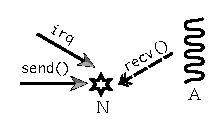
\includegraphics[width=\textwidth]{signal1}
        \caption{Notification}
        \label{f:signal1}
    \end{subfigure}%
    \begin{subfigure}[h]{0.48\textwidth}
        \centering
        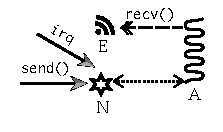
\includegraphics[width=\textwidth]{signal2}
        \caption{Bound notification}
        \label{f:signal2}
    \end{subfigure}
    \label{f:signal}
    \caption{Signals via a notification object. See \Cref{f:legend-1} for the legend.}
\end{figure}


\Cref{f:signal1} shows signal handling, where a thread A receives a signal and an interrupt at the
same time. In this case, the interrupt handler has a badged capability to the notification object,
$N$, as does the signaller. Both badges will be combined with a bitwise OR and delivered to the
receiver.

Signals can also be received by threads waiting on \gls{IPC}, as shown in \Cref{f:signal2}. A
\gls{TCB} object is bound to a notification object, establishing a link between them. Badges can be
used to determine whether a message was received from the endpoint or a signal on the notification object.

\subsection{System calls}

Over the last few sections we have indirectly presented several system calls for \gls{IPC} and
signalling. \Cref{t:system-calls} shows all the system calls available in \selfour. Communication
with the kernel itself is modelled as \gls{IPC} by using \texttt{call()} on kernel object
capabilities. Each capability has a set of \emph{invocations} which allow for methods on that object
to be used \eg binding a \gls{TCB} and notification object.

\begin{table} 
    \centering
    \rowcolors{2}{gray!25}{}
    \begin{tabular}{lp{0.6\textwidth}}\toprule
        \emph{System call} & \emph{Description} \\\midrule
        \texttt{send}      & One-way blocking \gls{IPC} or non-blocking signal.\\
        \texttt{nbsend}    & One-way non-blocking \gls{IPC} or non-blocking signal.\\
        \texttt{recv}      & Block waiting for a message or signal. \\
        \texttt{nbrecv}    & Poll for a message or signal. \\
        \texttt{call}      & Send an IPC and wait for a reply, or invoke the kernel. \\
        \texttt{reply}     & Send a message to the resume capability in the TCB CNode.\\
        \texttt{replyrecv} & \texttt{reply} and \texttt{recv} combined in one system call.\\
        \texttt{yield}     & Surrender current timeslice. \\
        \bottomrule
    \end{tabular}
    \caption{\selfour system call summary.}
    \label{t:system-calls}
\end{table}

\subsection{Thread states}

\begin{figure}[h!tb]
    \centering
    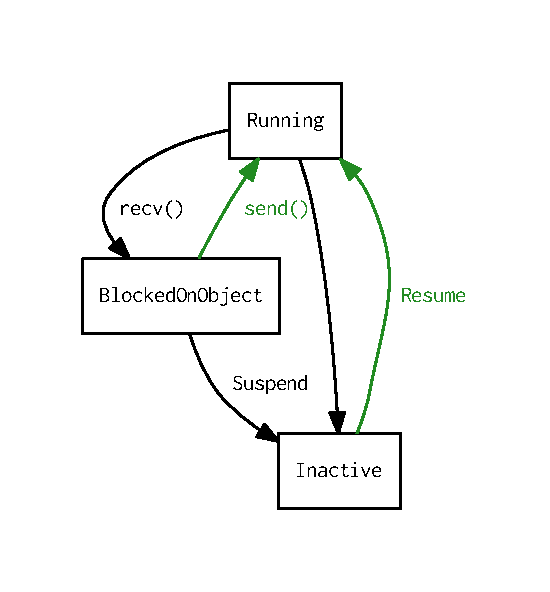
\includegraphics[width=1.1\textwidth]{thread_state}
    \caption{Thread state transitions in \selfour}
    \label{f:thread_state}
\end{figure}


\section{Scheduler}

The scheduler in \selfour is priority-based round-robin with 256 priorities (0 --- 255), implemented as an array of lists: one list of ready threads for each priority level. 
At a scheduling decision, the kernel chooses the head of the highest-priority, non-empty list, and
removes it from the relevant scheduler queue, which is referred to as \emph{Benno Scheduling}.
The kernel previously used \emph{lazy scheduling}, leaving the current thread in its run queue, however this was replaced in favour of Benno scheduling to reduce the WCET of the kernel. 
This is different to a previous kernel implementation which left the currently running thread in its run queue, however this increased the kernels \gls{WCET} and was removed.

Scheduling decision complexity is $O(1)$ as a two-level bit field tracks the highest priority with a runnable thread.

Kernel time is accounted for in ticks, with a static tick length defined at compile time (CONFIG\_TIMER\_TICK\_MS).
Threads have a timeslice field which represents the number of ticks they are eligible to run. 
This value is decremented every time a timer tick is handled, and when the timeslice is exhausted the thread is appended to the relevant scheduler queue, with a replenished timeslice.
The reload value of the timeslice is also defined at compile time (CONFIG\_TIME\_SLICE).

In an unrealistically simple system, where threads run at the same priority and do not communicate, it is possible to analyse temporal behavior on \selfour: threads will run for the timeslice value in round-robin order.
However, the allocation of ticks to threads is not actually that simple due to yield behaviour, preemption and \gls{IPC}. 

\subsection{Priorities}

Like any priority-based kernel without temporal isolation mechanisms, time is only guaranteed to the highest priority threads.
Priorities in \selfour act as informal capabilities: threads cannot create threads at priorities higher than their current priority, but can create threads at the same or lower priorities.
If threads at a higher priority levels never block, lower priority threads in the system will not run.
As a result, a single thread running at the highest priority has access to 100\% of processing time.
However, even this becomes unclear once there is more than one thread at a priority: if two threads are running, they can both access 50\% of processing time.
If one of two threads blocks, the other gets 100\% of processing time and vice versa.
There is no way to enforce a certain processor allocation and how CPU time a thread receives is up to priorities and the behavior of other threads in the system, which is impossible to guarantee.

\subsection{Accounting}
% I think this should move to the design section?
Due to the tick-based nature of the \selfour scheduler, when ticks are accounted complicates the
scheduling as the precision is reduced to the tick granularity, and described in
\cref{s:tick-v-tickless}.

Similarly, the \texttt{yield} system call will not alter the timeslice of the current thread, and
only donates a portion of the current tick to the next thread in the round-robin scheduler. 

\subsection{Domain scheduler}

A recent addition to the \selfour kernel adds the ability to guarantee complete temporal isolation and deterministic scheduling between sets of threads, using the concept of scheduling \emph{domains}.
Threads are assigned to domains, each of which has a separate array of lists of threads over the priority range.
Each domain runs for a fixed amount of ticks, and domains are scheduled sequentially and deterministically.
Cross-domain \gls{IPC} is delayed until a domain switch, and \texttt{yield} between domains is not
possible. When there there are no threads to run while a domain is scheduled, a domain-specific idle thread will run until a switch occurs.

The domain scheduler can be leveraged to achieve temporal isolation however since domains cannot be
preempted, it is only useful for cyclic, non-preemptive scheduling with scheduling order and
parameters computed-offline.
In such a scenario each real-time task could be mapped to its own domain, and each task would run for its specified time before the domain scheduler switched to the next thread.
Any unused time in a domain would be wasted, and spent in the idle thread.

However, in such a scheduler is only suitable for closed systems and results in low system utilisation.
Dynamic real-time applications with shared resources and high system utilisation are not compatible
with the domain scheduler, as they require preemption.

\section{RT support}

We introduced basic \selfour concepts and terminology, and investigated mechanisms that effect
timing behaviour in the kernel: the scheduler, priorities, yield and IPC. 
In this section we will look at how real-time scheduling could be implemented with those mechanisms.

There are several options for implementing a real-time scheduler in the current version of \selfour: leveraging the domain scheduler, using the priority scheduler or implementing a scheduling component to run at user-level. 
As the previous section established, the domain scheduler offers low utilisation for strictly closed
systems with strict temporal partitioning and no preemption, so is clearly insufficient.

The priority scheduler could be leveraged to implement a rate-monotonic scheduler.
However, this requires complete trust in every thread in the system, as there is no mechanism for temporal isolation: if one thread executes for too long, other threads will miss their deadlines.
Essentially the only thread with a guaranteed CPU allocation is the highest priority thread, which under rate-monotonic priority assignment is not the most critical thread in the system, but the thread with the highest rate.
Additionally, periodic threads driven by timer interrupts rather than events would need to share a user-level timer.

\begin{table}
	\centering
	\begin{tabular}{lp{2cm}p{2cm}p{2cm}p{2cm}} \toprule
        & \emph{Temporal isolation} & \emph{Utilisation} & \emph{Low kernel overheads} &
        \emph{Dynamic}\\
        \midrule
Domain scheduler          & \yes               & \no         & \yes        & \no    \\
Priority scheduler        & \no                & \yes        & \yes        & \yes   \\
Trusted timer component   & \yes               & \yes        & \no         & \yes   \\
        \bottomrule
	\end{tabular}
	 \caption{Comparison of existing \selfour scheduling options -- nothing ticks all of the boxes.}
	 \label{tab:nothing-ticks-all-boxes}
\end{table}


To build a dynamic system with temporal isolation and high CPU utilisation, one could implement a trusted timer component at user-level.
This component would be the highest priority thread in the system, and could pause threads to prevent them from overrunning their assigned rate.
However, since the timer component would need to maintain accounting information and track the currently running thread, it would need to be invoked for every single scheduling operation.
This is prohibitively expensive, as it results in doubled context switching time and increased number of system calls for thread management.

\Cref{tab:nothing-ticks-all-boxes} shows a comparison of all of the available scheduling options in the current version of \selfour -- no option provides all of the qualities we require.
Clearly, the kernel needs something more. 
In the next section we will our model for a more principled approach to time by extending the
baseline \selfour model presented in this chapter. We incorporate using the principles of resource kernels and with the aim of support diverse task sets, including those for mixed-criticality systems.

